% Question  ##################################################################################################################
\section{Question 4}\label{ssec:pt2q4}
\textbf{Cryptocurrencies and blockchain are amongst the most currently discussed topics in the Fintech world.}
% END Question  ##############################################################################################################

% Question (i) ###############################################################################################################
\subsection{Q4 (i)}\label{sssec:pt2q4i}
\textbf{Provide, technically feasible situations, where you as an expert would suggest the adoption of blockchain technology. In your answer explain the cons and pros of using blockchain viz-a-viz other commonly used architectures.}

\noindent
Although Blockchain is an innovative technology, it is not always feasible to implement every solution on to the chain.  One of the main advantages of Blockchain is that it allows the use of decentralization meaning that you don’t need a middleman/server (removing the dependency of a central server or database) to communicate/transact with and it allows a user to directly cut off the middleman. Another advantage is that some chains allow for code to hold value similarly to Ethereum’s smart contracts. For the purposes of this question we will discuss feasible solutions which can be implemented on to the chain and we assume that the Ethereum’s network will be used, since there are many variations which have different functionalities, but most of the features described here are implemented in other chains which allow programmability (Generalised Blockchains). Another great advantage when using the chain is that transactions are immutable meaning, once they are written, they cannot be changed and are permanently stored on the chain. 

\noindent
The following are some situations where we believe blockchain could be useful/feasible:                     

\noindent
\textbf{Registry Systems}

\noindent
An example where we think that Blockchain can be useful is in situations where someone needs to register something. For example, let’s look at land and car registry. A system built using the Blockchain can allow for land registries or car registries to be saved on the chain. This will allow the ones using the system to view ownership, previous owners and property/car rights from data saved on the chain. Due to the immutability property of the Blockchain, data cannot be tempered with, which is very important in this situation.

\noindent
Clients do not have to trust the ones who take care of the system, as in itself data cannot be changed.  Compared with the traditional systems of using a database, where a server can be vulnerable to attack, and data can be changed for the benefit of an attacker. Such solution can help mitigate property fraud. Although this solution allows for immutability, which may be a great advantage, all the data saved on the chain is publicly available. Let’s say that a property ownership is linked to an owner via an address, once someone can link this address to a person, they can easily know what property or car he/she owns or previously owned. The use of private chains can help with this situation, but again every node in this chain has the capability of doing the same thing described. 

\noindent
An example where ownership of a property is saved on the chain is ‘CryptoKitties’ \cite{cryptokitties} where users purchase, breed and collect virtual cats. So, similar applications where there is a need for ownership of a virtual property, such as game, can be implemented in the same manner. In the case of games there might be a problem with scalability as the Ethereum network can only process about 25 tx/s and you don’t want to stop a player from purchasing a virtual property just because the system is under a heavy load. 

\noindent
Some other feasible situations which were not discussed: Money (cryptocurrencies), Exchanges, Crowd Sourcing, Markets and Automating regulatory compliance. 

\noindent
Overall the pros and cons described in the such situations above, can be generalized as follows: 
\noindent
\textit{Blockchain}

\noindent 
\textbf{Pros:}

\begin{itemize}
    \item Trustless: No party needs to trust the other party.
    \item Immutability: Once the data is written it cannot be changed.
    \item Security against DoS attacks as it would be expensive to conduct such an attack. 
    \item Decentralization: All of the nodes contain a copy of the chain, so if one node fails the system can still continue to run.
\end{itemize}

\noindent 
\textbf{Cons:}

\begin{itemize}
    \item Cost: Each transaction comes with a fee (Miner Fees). 
    \item Secrets: In most of the chains it is very difficult to store secrets without a third party interference. 
    \item Scalability: The state of public Blockchains right now do not scale well (delays under massive amounts of transactions.)
    \item 51\% Attacks: Public Blockchains using PoW can be targeted with colluding malicious miners, which can end up in 'Double Spending'. 
\end{itemize}

\noindent
\textit{Commonly used Architectures}

\noindent 
\textbf{Pros:}
\begin{itemize}
    \item Secrets: Can store secrets on the system without public access by anyone.
    \item Cost: A transaction does not require a cost (No Miner Fee). 
    \item Time: Transactions do not need miners to be processed. 
    \item Scalability: Most commonly used architectures are easily scalable (if written well). 
\end{itemize}

\noindent 
\textbf{Cons:}
\begin{itemize}
    \item Mutable: Data is mutable and can be tempered with.
    \item Attacks: Prone to DoS attacks. 
    \item Trust: The client has to trust the service. 
    \item One point of failure, if the system fails a service is unusable (although this is mitigated by having backup servers ). 
\end{itemize}

\noindent
Before implementing a system using Blockchain we believe that the following questions must be answered before even considering it: 
\begin{itemize}
  \item Is it feasible to use a public database where multiple parties can access it ? (Yes) 
  \item Is there a need for an intermediary or this could be cut entirely ? (Yes)
  \item Are the transactions done on the system dependent on each other ? (Yes)
  \item Is it a requirement for the system to have immutability ? (Yes)
  \item Can the system wait for the transactions to be processed ? (Yes)
\end{itemize}

% END Question (i) ###########################################################################################################

% Question (ii) ##############################################################################################################
\subsection{Q4 (ii)}\label{sssec:pt2q4ii}
\textbf{Explain proof-of-work and how the algorithm permits decentralised concensus.}

\noindent
PoW (proof-of-work) is the consensus algorithm used in the Bitcoin \cite{nakamoto2008bitcoin} network, although there are other networks which also use such algorithm, i.e the Ethereum network \cite{wood2014ethereum}. The PoW concept was introduced in HashCash were it was used to limit email spam \cite{dwork1992pricing} and DoS attacks \cite{back2002hashcash} by making the processor use some of the processing power to compute a hashcash stamp to be added to the header of an email, so that the sender can prove that it did some work before sending an email. 

\noindent
In the case of cryptocurrencies, the algorithm is used to combat Byzantine Failures in a decentralized network and to reach consensus between the nodes connected to the network. This is a probabilistic approach to solve the Byzantine Generals Problem, a problem in decentralized networks described by Lamport \cite{lamport1982byzantine}. Such algorithm is basically a cryptographic puzzle which each miner on the network is trying to solve. Now we will be describing how PoW consensus works in the Bitcoin network. 

\noindent
To correctly explain this mechanism, first we need to define some data structures used in the network, to be able to know what a block header is. Each block in the blockchain contains a data structure called a Merkle tree. This structure is used to hold the transactions in a specific block. For simplicity reasons let assume that the leaf node in the Merkle tree shown in Fig.~\ref{fig:pow_1} is a transaction. The parent node is than composed of two pairs of hashes generated from the leaf nodes. The parent of the parent of the leaf nodes is composed of two other pairs of hashes and this process keeps on going until you reach the root node which has the hash generated from this process. 

\begin{figure}[H]
\centering
  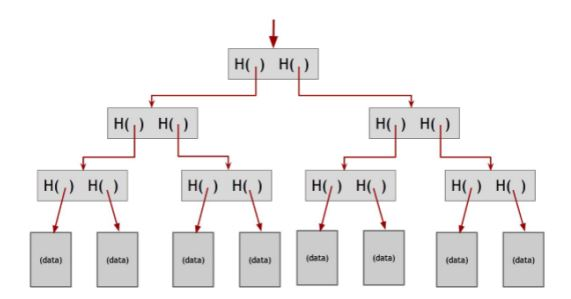
\includegraphics[scale = .70]{imgs/merkle_tree.JPG}
  \caption{A visual representation of a Merkle tree.}
  \label{fig:pow_1}
\end{figure}

\noindent
In the block header you will have the following components; Bitcoin Version Number, Previous Block Header Hash, Hash of the root node for the Merkle Tree, The block timestamp (unix), Difficulty for the target block and the nonce. What happens in PoW is that miners use their computing power to find a nonce (a numeric value) which when hashed (SHA256) with the block header would create a value with leading zeros.  This hash is valid if the value is below the target. The difficulty can be adjusted, in fact in the Bitcoin network it is adjusted every 2016 blocks. 

\noindent
Once a miner solves this puzzle the block is propagated through the network so other miners can start working on a new block. Since the blocks have a hash pointer to the previous block all blocks are dependent on the previous one and if you had to visualize this you will see a chain of blocks as shown in Fig.~\ref{fig:pow_2} hence the name blockchain. The more computation power a miner has the more nonce values this node can try. The mining process is also incentivised, meaning that when a miner solves the puzzle it will be rewarded with bitcoin (in fact this is how new bitcoin is created although the total supply is capped). The longest chain in the network is the chain which the nodes agree on, meaning the blocks (transactions) which are valid to the network. This mechanism also is way to try and handle the ‘Double Spending Problem’ described in Satoshi Nakamoto paper \cite{nakamoto2008bitcoin}. 

\begin{figure}[H]
\centering
  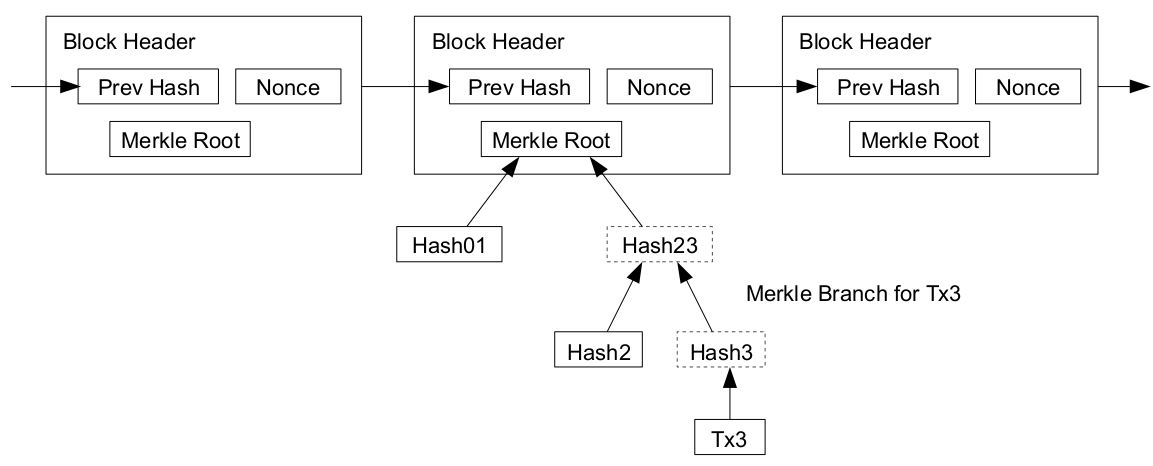
\includegraphics[scale = .50]{imgs/blockchain.JPG}
  \caption{A visual representation of the Blockchain.}
  \label{fig:pow_2}
\end{figure}

\noindent
Such mechanism only works if most of the hashing power belongs to none malicious miners. When you have 51\% of the miners who are colluding and acting maliciously it is guaranteed that they can control the network and can double spend their coins. In fact, this attack was done on the network of the cryptocurrency called ‘Bitcoin Gold’ were they doubled spent their value to defraud exchanges \cite{51attack}.  

\noindent
The PoW mechanism permits decentralise consensus for the following traits; Every full node can verify each transaction independently, each block which is propagated by the miner can be verified independently, transactions can be aggregated independently into new blocks (mining nodes) and a solution is provided if two miners propagate a block at the same time (longest chain) and every miner node can participate to take part of the mining process (although the use of mining pools goes against Satoshi’s vision, since hashing power is becoming more centralized). 

% END Question (ii) ##########################################################################################################

% Question (iii) #############################################################################################################
\subsection{Q4 (iii)}\label{sssec:pt2q4iii}
\textbf{Your group of friends happen to be football fanatics. You decide to utilise a smart contract to manage bets with your friends for an upcoming tournament. Each participant will need to guess the winner of the competition and is allowed to log his preferred team only once (1 bet allowed). The participants will have to place their bet before the first tournament game – Feb 1st, 2019 - beyond which the smart contract will not allow any further bets.}

\noindent
\textbf{Each participant would need to put 10 Euro in the pot. To keep things simple, you decide that the pot will be managed externally using normal fiat money, however you believe that for transparency purposes a balance showing the total pot collected should be available on the contract.}

\noindent
\textbf{Once the official winner is known, you as the organiser will update the contract. The contract should not permit setting the winner before end of competition -28th of Feb, 2019. Each participant can query the contract and check the amount won by him (if any), depending on (i) whether he guessed or not and (ii) whether he was the only one guessing the winning team (if not, then the total money won will be Total pot divided by total number of winning participants).}

\noindent
\textbf{Assume that teams are numbered 1-10 (assuming 10 teams).}

\noindent
\textbf{Create a smart contract that can manage this use case. Provide source code of the contract with explanations of how the problem is approached.} 

\noindent
Code for this task is in \textit{‘src/solidity/football\_competition\_truffle’}. Inside the location provided there is a folder called \textit{‘contracts’} were the smart contract called ‘FootballCompetition.sol’ is used to manage this use case. Also, there is a folder called \textit{‘python’} which has a script called ‘chain\_comp.py’ which is used to test the contract which was written. 

\noindent
Let’s explain the code inside the ‘FootballCompetition.sol’. First off, the contract inherits from an open source contract called ‘Ownable.sol’ from OpenZepplin \cite{solidity:openzepplin} which basically is a contract which gives some functionality to manage the owner modifier for the contract. This contract gives us functionality such as checking that the owner of the contract can only access a specific function and some other functions such as transferring ownership to another address. The ‘Ownable.sol’ is located in: 

\noindent
\textit{‘src/solidity/football\_competition\_truffle/installed\_contracts/zepplin/contracts/ownership’}.

\noindent
After doing so three different structs were written which will be utilised later in the contract. These can be shown in Fig.~\ref{fig:comp_sol_1}. All variables in the structs are commented so it is self-explanatory for what the variables will be used for. Also, the contract was written in a way that there could be multiple competitions created by different organizers/addresses, this was done to make the use-case more dynamic and can accept multiple competitions. 

\begin{figure}[H]
\centering
  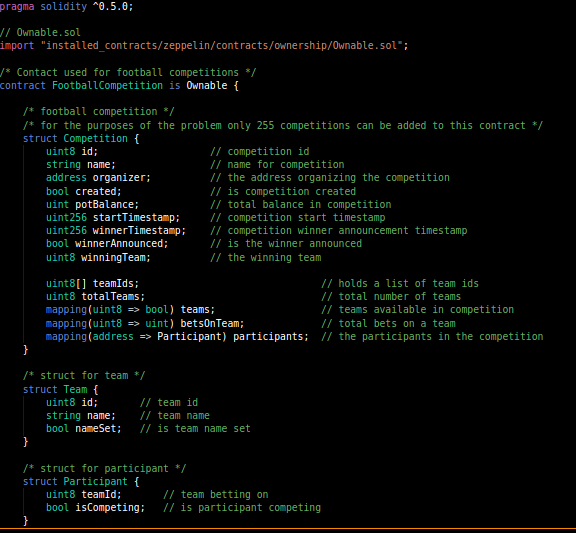
\includegraphics[scale = .70]{imgs/comp_sol_1.png}
  \caption{Three different structs in the 'FootballCompetition.sol' contract.}
  \label{fig:comp_sol_1}
\end{figure}

\noindent
Then variables for the contract were defined and again from the comments one can know what the use for these variables is. In the constructor the count for the competition and teams is set to 0, as we want them to be 0 once the contract is deployed. Both the variables and constructor can be shown in Fig.~\ref{fig:comp_sol_2}. Some modifiers which will later be used were also define and these can be shown in Fig.~\ref{fig:comp_sol_3} (the comments explain the use for each modifier).

\begin{figure}[H]
\centering
  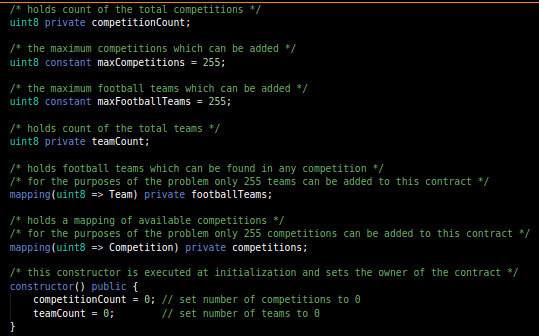
\includegraphics[scale = .70]{imgs/comp_sol_2.png}
  \caption{Variables and constructor for 'FootballCompetition.sol' contract.}
  \label{fig:comp_sol_2}
\end{figure}

\begin{figure}[H]
\centering
  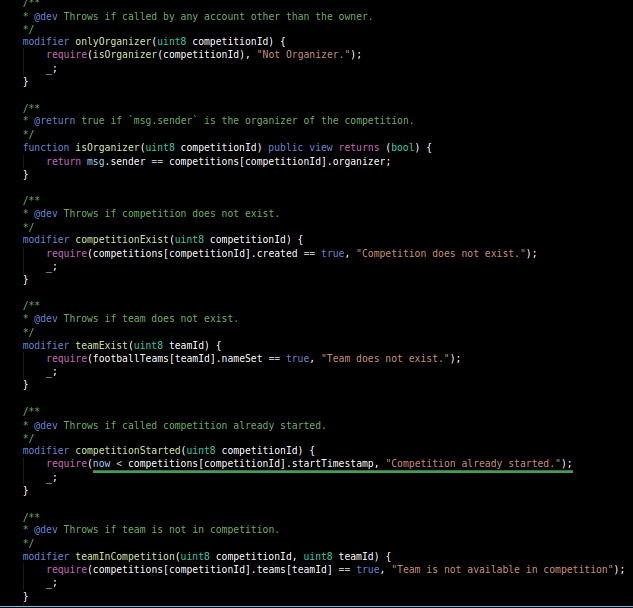
\includegraphics[scale = .65]{imgs/comp_sol_3.png}
  \caption{Modifiers for 'FootballCompetition.sol' contract.}
  \label{fig:comp_sol_3}
\end{figure}

\noindent
The first two functions written in the contract as shown in Fig.~\ref{fig:comp_sol_4}, just outputs the number of teams and competitions available in the contract. This can later be used to query the total number of teams available to select from, when organizing a new competition, while the other gives us the number of competitions available in the contract. This is a common design pattern used in smart contracts, since when you want to show the available teams or competition from a client, first you get the count and then call the get team or get competition to view the details for every team or competition available (ids are set incrementally). This is done because using unbound arrays in the EVM can have a high gas cost. 

\noindent
The other function shown in Fig.~\ref{fig:comp_sol_4} (‘addTeam’) lets the owner (the one who deployed the contract) to add a new team. A name for the team must be specified and this was written in this way, because we assume that the contract can have different teams to select from to when creating a new competition. Another consideration which was taken, is that a team name cannot be edited for transparency/trust reasons (we don’t want the owner of the contract to change the name of the team with a specific id as this can cause issues when the winner or a bet is set in previous or active competitions). Once a team is added it is saved in the mapping 'footballTeams' and the variable/bool ‘nameSet’ is set to true. This is a common design pattern in solidity, whenever you need to check if a key exists in the mapping ('teamExists' modifier).

\begin{figure}[H]
\centering
  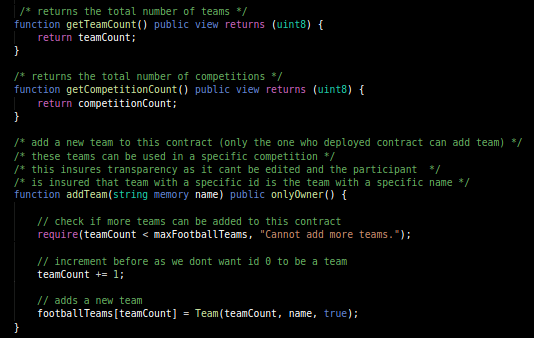
\includegraphics[scale = .75]{imgs/comp_sol_4.png}
  \caption{First three functions in 'FootballCompetition.sol' contract.}
  \label{fig:comp_sol_4}
\end{figure}

\noindent
The next function is the ‘getTeam’ as shown in Fig.~\ref{fig:comp_sol_5}, and this returns details about a team with the specified id. Such function can be called in conjunction with the get count for the teams from a client to get all the available teams, which can be selected when creating a competition (as described due to unbounded arrays). 

\begin{figure}[H]
\centering
  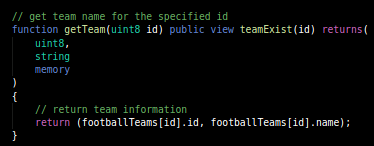
\includegraphics[scale = .75]{imgs/comp_sol_5.png}
  \caption{Get team details function in 'FootballCompetition.sol' contract.}
  \label{fig:comp_sol_5}
\end{figure}

\noindent
One of the most important function in the contract is the ‘addCompetition’ function as shown in Fig.~\ref{fig:comp_sol_6} and this lets anyone to create a new competition which other addresses can join and bet in. The dates when the competition starts, and end must be specified together with the name of the competition. The address who created the competition is also noted and once this function is called the newly created competition is saved in the mapping. The created variable/bool is used in similar ways as the Team struct, which is to check if a competition exists (‘competitionExists’ modifier). 

\begin{figure}[H]
\centering
  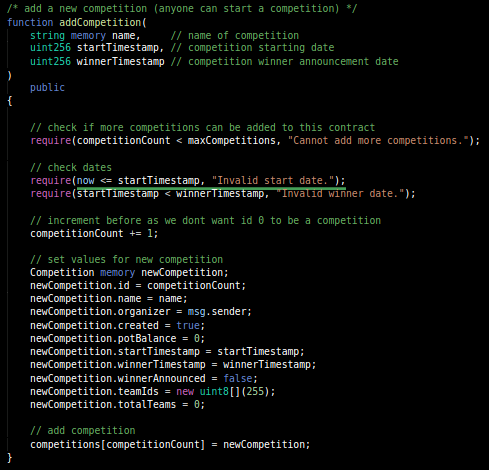
\includegraphics[scale = .75]{imgs/comp_sol_6.png}
  \caption{Add competition function in 'FootballCompetition.sol' contract.}
  \label{fig:comp_sol_6}
\end{figure}

\noindent
The ‘getCompetition’ function works similarly as the described function  ‘getTeam’. This can be used to check the details for available competitions stored on the chain and this is shown in Fig.~\ref{fig:comp_sol_7}. Such details include the available teams an address can bet on for this particular competition. 

\begin{figure}[H]
\centering
  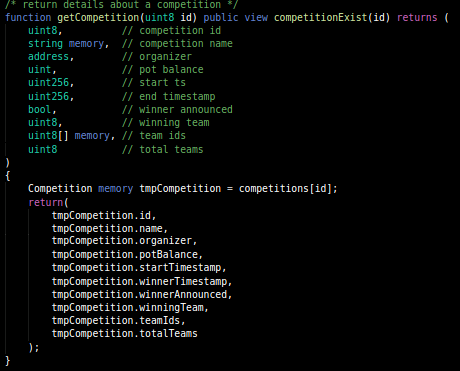
\includegraphics[scale = .75]{imgs/comp_sol_7.png}
  \caption{Get competition details function in 'FootballCompetition.sol' contract.}
  \label{fig:comp_sol_7}
\end{figure}

\noindent
Another important function which can only be accessed by the one who created the competition (‘onlyOrganizer’ modifier) is the ‘addTeamToCompetition’ as shown in Fig.~\ref{fig:comp_sol_8}. This lets the organizer to add teams which will be competing in the created competition and this team must be one of the available teams which are saved on the chain (‘teamExists’ modifier). Note that an organizer cannot add new teams to the competition if the event already started and another restriction added, is that the organizer cannot add already existing teams in the competition.

\begin{figure}[H]
\centering
  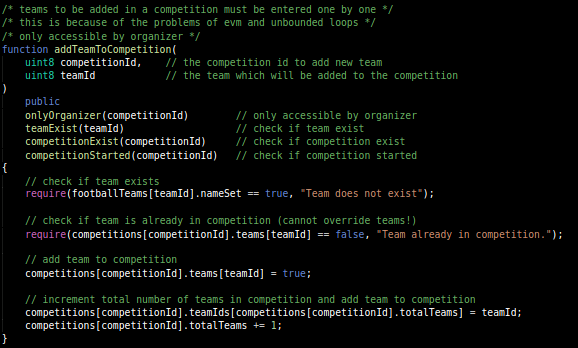
\includegraphics[scale = .75]{imgs/comp_sol_8.png}
  \caption{Add team to competition function in 'FootballCompetition.sol' contract.}
  \label{fig:comp_sol_8}
\end{figure}

\noindent
To join an existing competition the function ‘joinCompetition’ was created as shown in Fig.~\ref{fig:comp_sol_9}. This allows an address to put a bet from the teams in the competition and this restricts the address to one bet only. Also no one can join the competition if the event already started (‘competitionStarted’ modifier). It is also important to note that the count for each bet done on a specific team is noted in the variable ‘betsOnTeam’ inside the Competition struct. This was done to easily and efficiently split the winnings in a function which will be discussed soon. 

\begin{figure}[H]
\centering
  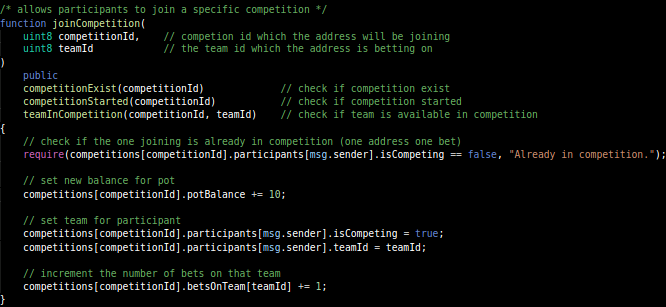
\includegraphics[scale = .75]{imgs/comp_sol_9.png}
  \caption{Join competition function in 'FootballCompetition.sol' contract.}
  \label{fig:comp_sol_9}
\end{figure}

\noindent
An organizer then can set the winner for the competition by calling the ‘setWinningTeam’ function as shown in Fig.~\ref{fig:comp_sol_10}. The winner can only be set if the end date has passed as shown in the second require in the function. The last function which was written lets any address which was competing to check if they won anything. This could be called once the winning team is set. Such function is shown in Fig.~\ref{fig:comp_sol_11}.

\begin{figure}[H]
\centering
  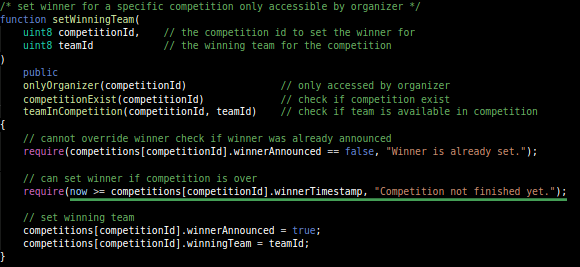
\includegraphics[scale = .7]{imgs/comp_sol_10.png}
  \caption{Set winner for competition function in 'FootballCompetition.sol' contract.}
  \label{fig:comp_sol_10}
\end{figure}

\begin{figure}[H]
\centering
  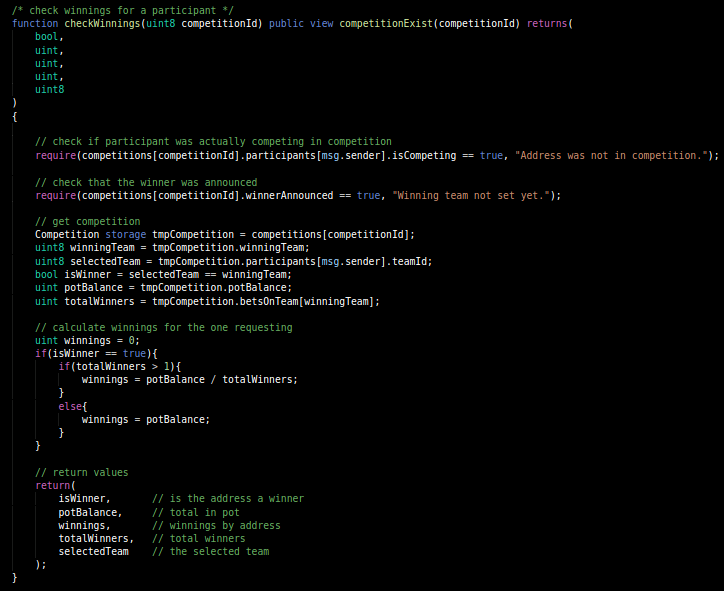
\includegraphics[scale = .6]{imgs/comp_sol_11.png}
  \caption{Check winnings for competition function in 'FootballCompetition.sol' contract.}
  \label{fig:comp_sol_11}
\end{figure}

\noindent
Once the contract was written it was compiled and deployed from python. Some tests were done to make sure everything works well. One thing to keep note of, is the time on the chain is set to UTC so the timestamps send to create a competition must be converted to UTC for this contract to work properly. The test was conducted using the current timestamp and add 5 seconds to the start timestamp and 10 seconds to the end timestamp. Then a delay is set in python, and this was done to make sure that the timestamp checks are working correctly. Finally, we would like to add that this contract can be used for the use case specified in this question. Fig.~\ref{fig:comp_sol_12} shows the final output for the test, which is a call to the function which checks the winnings for a participant (first 6 participants are shown using a loop). 

\begin{figure}[H]
\centering
  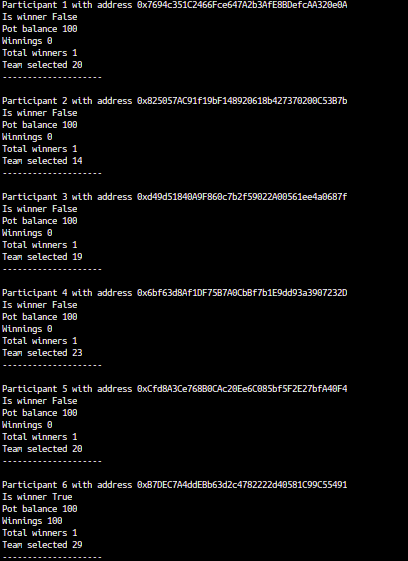
\includegraphics[scale = .65]{imgs/comp_sol_12.png}
  \caption{Final output of winnings when testing the contract.}
  \label{fig:comp_sol_12}
\end{figure}

% END Question (iii) #########################################################################################################
